\scanpage{8}
\mspage{6}
\margin{\figure{\begin{tikzpicture}\draw (0,0).. controls (.14,-.22) and (.39,-.45) .. (.5,-.65).. controls (.51,-.68) and (.52,-.72) .. (.51,-.74);\end{tikzpicture}}}

\begingroup\setbox0=\hbox{11}\hbox{\rlap{\begin{tikzpicture}[overlay,baseline=0pt]\draw[line width=.45pt] (-5pt,-6pt) .. controls (-12pt,4pt) and (-4pt,21pt) .. (8pt,22pt) .. controls (\dimexpr\wd0+9pt\relax,23pt) and (\dimexpr\wd0+12pt\relax,1pt) .. (\dimexpr\wd0+6pt\relax,-5pt) .. controls (8pt,-12pt) and (-2pt,-10pt) .. (-5pt,-6pt);\end{tikzpicture}}\box0}\endgroup{}\quad pg101\quad $\ell-6$.\quad Dire où on trouve que Néron commute à $S\mapsto\widehat S$.

\bigskip
\noindent

\begin{tikzpicture}[baseline=0pt,overlay,x=1em,y=1ex]
\draw[gray] (6.4,3.7) .. controls (7.2,2.3) and (7.8,.1) .. (7.6,-1.7)
.. controls (6.6,-3.5) and (-.6,-4.4) .. (-.7,-2.2)
.. controls (-1.2,0) and (-.2,1.7) .. (1.0,2.3)
.. controls (3.6,4.1) and (6.8,6.2) .. (6.5,3.9);
\end{tikzpicture}
\raisebox{-1.5ex}[0pt][0pt]{\makebox[0pt][l]{\textcolor{gray}{que\ \raisebox{2.3ex}{faire ?}}}}
\hspace*{3.5em}pg103\qquad Le renvoi au courage du lecteur est désagréable --

\medskip
Si j'ai bien compris, tu affirme que prolonger une \unsure{biextension} à $A\times A'$ est ``la $\hat{\mathrm m}$ chose'' que de la prolonger aux $ {}_{\ell^\infty}A\times{}_{\ell^\infty}A'$.

\margin{7}
